\scanpage{5}

\diagram{\begin{tikzcd}[ampersand replacement=\&,column sep=1.4em]
{\mathbb Z[\mathbb F_{\unsure{n-2|n\,2|n-1}}]}
 \& {\mathbb Z[\mathbb F_{n-1}]}\arrow[l]
 \& {\mathbb Z[F_n]}\arrow[l,"{t_n-s_n}"]
 \& {\mathbb Z[\mathbb F_{n+1}]}\arrow[l]
\end{tikzcd}}
% Detached nonlinguistic ink immediately after the chain, source bbox [1174,120,1195,136].
% Its horizontal bridge, two upright lobes and lower-right foot are not a simple dot or comma.
\figure{\begin{tikzpicture}[x=.12em,y=.12em,line width=.8pt,line cap=round,line join=round]
\draw (0,0)--(0,.9)--(.35,.6)--(.7,.4)--(1.4,.7)--(1.4,1.2)
 (0,.15)--(1.5,.15)--(1.5,-.45)--(2,-.45)--(1.8,-.2);
\end{tikzpicture}}
% Unattached bent ink strokes below the right end of the chain; no linguistic reading assigned.
\figure{\begin{tikzpicture}[x=.1em,y=.1em,line width=.35pt,line cap=round]
\draw (0,0)--(.4,-.8)--(1,-1.2);
\draw (1.15,-1.3)--(1.4,-1.4);
\draw (2.7,-.2)--(3.2,.1);
\end{tikzpicture}}

\[
\begin{aligned}
D_n&\longrightarrow X &\quad&\deleted{D_n}\,\raisebox{1.1ex}{\(\cdot\)}\\
\bigl\{x&\in F_n && =
\end{aligned}
\]

% The source's first and last small arguments lack a separate opening parenthesis.
% The square-ended low bracket occupies source [265,630,588,658], below only the left part.
\figure{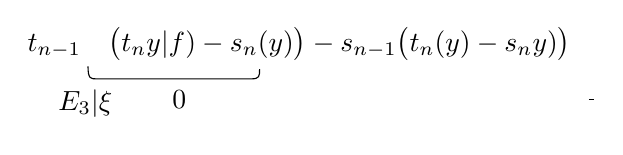
\begin{tikzpicture}[line width=.4pt]
\node[anchor=west,inner sep=0pt] (eq) at (0,0)
 {$t_{n-1}\quad\bigl(t_n\unsure{y|f})-s_n(y)\bigr)-s_{n-1}\bigl(t_n(y)-s_n y)\bigr)$};
\draw ([xshift=2.2em,yshift=-.8em]eq.west)
 .. controls ([xshift=2.2em,yshift=-1.25em]eq.west) and ([xshift=2.3em,yshift=-1.25em]eq.west)
 .. ([xshift=2.5em,yshift=-1.25em]eq.west)
 -- ([xshift=8.1em,yshift=-1.25em]eq.west)
 .. controls ([xshift=8.4em,yshift=-1.25em]eq.west) and ([xshift=8.4em,yshift=-1.15em]eq.west)
 .. ([xshift=8.4em,yshift=-.9em]eq.west);
\node at ([xshift=5.5em,yshift=-2em]eq.west) {$0$};
\node at ([xshift=2.1em,yshift=-2.15em]eq.west) {$\unsure{E_3|\xi}$};
% A short detached ink dash at source [1168,696,1180,705].
\draw ([xshift=20.3em,yshift=-2em]eq.west)--([xshift=20.48em,yshift=-2em]eq.west);
\end{tikzpicture}}

\[
\begin{array}{cc}
\underset{\smile}{F}_0 & \unsure{F|\mathbb F}_1\\[.6em]
F'_0 & \mathbb F'_1\\
\unsure{\prime|1}&
\end{array}
\]
\diagram{\begin{tikzcd}[ampersand replacement=\&,column sep=1.7em,row sep=1.3ex]
\&\& \unsure{s|f}\&t\arrow[l]\\
{\substack{\exists\,\deleted{u}s,u'\\s'}} \&
 f(s)\arrow[l] \& f_0(s) \& f_0(t)\arrow[l]
\end{tikzcd}}

\begin{flushright}
\begin{minipage}{.74\linewidth}
\(\bigl(C_i\bigr)\quad\forall w'\in\mathbb F'_i,\)
\deleted{si on \unsure{retient|retire}} \(\deleted{s}\exists w\in F_i.\) tel que
\(f(w)\sim w'\). De plus si \(i\geq1\), On peut
\par\noindent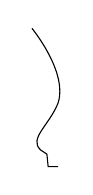
\begin{tikzpicture}[baseline=-2.3em,x=.45em,y=.5em,line width=.4pt]
\draw (0,5)..controls(1.7,3)and(2.6,1)..(2.1,-.4)
 ..controls(1.4,-2)and(-.3,-3)..(.7,-3.8)--(1.2,-4.1)--(1.3,-5)--(2.1,-5);
\end{tikzpicture}\begin{minipage}{.89\linewidth}
se donner d'avance \(u_{\unsure{i-1|i}}=s_i(w)\), \inserted{\(v_i=\)}\(t_i(w)\),
\inserted{de \(F_{i-1}\)} soumis aux seules conditions \deleted{de} que
\(f(u_{\unsure{i|1}})=u'_i\), \inserted{\unsure{rp|resp}}
\(f(v_i)=v'_i\)
et, \deleted{de} plus, si \(i-1\geq1\) i.e \(i\geq2\), \deleted{que}
\(s(u)=s(v),\ t(u)=t(v)\)
\end{minipage}

(NB on n'exige pas que \(\unsure{f|g}(u)=u'\))
\end{minipage}
\end{flushright}

\[
\begin{aligned}
\unsure{\Xi|E}_0\quad\text{\textcircled{\(\unsure{\mathrm a)|\mathrm b)}\)}}\quad&
\forall \text{\uline{\(s\)}}'\in F'_0,\quad \exists s\in\mathbb F_0,\ u\in\mathbb F'_1,\quad
f_0(s)\xrightarrow{u}s'\\[-.1em]
&\hspace{4em}\deleted{\pi_0(f)\ \text{surj}}\quad
-\pi_0(f)\ \text{\uuline{surj}}\\
\mathrm b)\quad&
\forall s,t\in F_0,\quad
\underset{\substack{\rotatebox{90}{\(\in\)}\\F'_1}}{u'}:f_0(s)\longrightarrow f_0(t),\\
&\exists u\in\mathbb F_1,\quad u:s\mathbin{-}t\qquad\pi_0(f)\ \text{inj.}
\end{aligned}
\]

\[
\begin{aligned}
\Xi_1\quad\text{\textcircled{\(\mathrm b')\)}}\quad&
\forall s,t\in\mathbb F_0,\quad
\underset{\substack{\rotatebox{90}{\(\in\)}\\F'_1}}{u'}:
 f_0(s)\mathbin{-} f_0(t),\\
&\exists u\in F_1,\quad u:s\mathbin{-}t,\quad
 f(u)\xrightarrow[\sim]{\ell}u'\\
&\deleted{\unsure{w|\exists\,w}\in F_2}\\
&\pi_0(f)\ \text{inj. et }\text{\uuline{\(\pi_1(f)\) surj}}
\end{aligned}
\]
% The wavy stroke in the preceding arrow is drawn across its shaft in the source.

\[
\begin{aligned}
\mathrm c)\quad&
\deleted{\forall s,t\in\unsure{\mathbb F_0|F_0},}\ u,v\in\unsure{F|\mathbb F}_1\quad
\begin{gathered}s_i(u)=s_1(v),\\[-.2em] t_1(u)=t_1(v)\end{gathered},\\
&\text{et }\underset{\substack{\rotatebox{90}{\(\in\)}\\\mathbb F'_2}}{w'}:
 f(u)\longrightarrow f(v),\quad
 \exists\underset{\substack{\rotatebox{90}{\(\in\)}\\\mathbb F_2}}{w}:
 \deleted{\unsure{f_1|f}}u\mathbin{-}v\\
&\pi_{\unsure{f|1}}(f)\ \text{inj.}
\end{aligned}
\]
% Source [470,1372,583,1508]: two arrows have separate endpoints, with gaps on both sides.
\figure{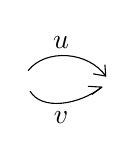
\begin{tikzpicture}[x=1.4em,y=1em,line width=.4pt,line cap=round,line join=round]
\draw (-1,.2)..controls(-.55,1)and(.55,.9)..(1,0);
\draw (.68,.08)--(1,0)--(.98,.4);
\draw (-.95,-.55)..controls(-.65,-1.25)and(.3,-1.05)..(.9,-.4);
\draw (.55,-.37)--(.9,-.4)--(.65,-.66);
\node at (-.15,1.2) {$u$};
\node at (-.15,-1.5) {$v$};
\end{tikzpicture}}

\[
\begin{aligned}
E_2\quad\text{\textcircled{\(\mathrm c'\)}}\quad&
\forall(u,v)\in\mathbb F_1,\quad
\begin{gathered}s_1(u)=s_1(v)\\[-.2em] t_1(u)=t_1(v)\end{gathered}
\quad\text{et }\underset{\substack{\rotatebox{90}{\(\in\)}\\\mathbb F'_2}}{w'}:
 f(u)\mathbin{-}f(v),\\
&\exists\underset{\substack{\rotatebox{90}{\(\in\)}\\\mathbb F_2}}{w}:u\longrightarrow v\ 
 \deleted{et}\ \text{tel que}\\
&w'\sim f(w)
\end{aligned}
\]
% Source [1981,1363,2342,1520]: asymmetric rounded grouping stroke, without a central brace peak.
\figure{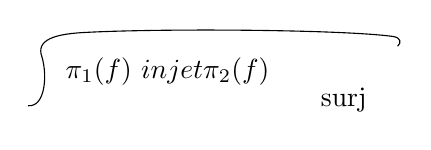
\begin{tikzpicture}[x=1em,y=1em,line width=.4pt]
\node[anchor=west] at (0,0) {$\pi_1(f)\ \text{inj et }\pi_2(f)$};
\node at (10.4,-1.05) {surj};
\draw (-1,-1.25)..controls(-.4,-1.3)and(-.3,-.2)..(-.5,.5)
 ..controls(-.75,1.15)and(0,1.35)..(1.1,1.4)
 ..controls(4,1.55)and(10.4,1.5)..(12.2,1.25)
 ..controls(12.45,1.2)and(12.5,1.05)..(12.35,.9);
\end{tikzpicture}}
% Source [1109,1538,1203,1657]: separated arc endpoints; lower right return; three detached dots.
% The vertical arrow passes between the w and its prime, not to the right of the prime.
\figure{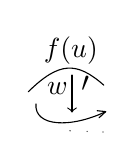
\begin{tikzpicture}[x=1.4em,y=1.1em,line width=.4pt,line cap=round,line join=round]
\draw (-1,0)..controls(-.2,1)and(.25,1)..(.95,.22);
\draw (-.8,-.4)..controls(-.85,-1.15)and(.1,-1.2)..(1,-.65);
\draw (.78,-.62)--(1,-.65)--(.83,-.85);
\node at (.1,1.35) {$f(u)$};
\node at (-.25,.12) {$w$};
\node at (.47,.25) {$\prime$};
\draw[->] (.13,.55)--(.13,-.68);
\fill (.08,-1.28) circle (.025em);
\fill (.52,-1.3) circle (.022em);
\fill (.93,-1.32) circle (.022em);
\end{tikzpicture}}
% archive sheet number: 4
% Pale rotated background impressions are present; no additional word was recoverable securely.
